\chapter{Results}
\label{chap:results}

\section{Data Preprocessing}
\label{sec:data_preprocessing}

Raw imagery and annotations gathered from diverse household environments exhibit substantial heterogeneity in camera resolution, spatial aspect ratios, ambient illumination, and occlusion profiles. To condition these inputs for deep convolutional object detection, an automated, deterministic preprocessing pipeline was formulated:

\begin{enumerate}
    \item \textbf{Supervisely-to-YOLO Annotation Transformation}: Annotation files in Supervisely JSON format were parsed to extract object polygon boundaries, exterior bounding vertices, and category tags. Vertex coordinates were mapped to normalized YOLO bounding box tuples:
    \begin{equation}
        [c, x_{\text{center}}, y_{\text{center}}, w, h]
    \end{equation}
    where $c \in \{0, 1, \dots, 8\}$ represents the zero-indexed class ID, and all spatial coordinates are strictly bounded within $[0.0, 1.0]$ relative to image dimensions $W$ and $H$. Invalid bounding boxes (e.g., zero width, coordinates outside frame boundaries, or corrupt coordinates) were filtered out automatically during validation.
    \item \textbf{Letterbox Aspect-Ratio Padding}: Direct non-uniform resizing introduces artificial aspect ratio deformation that degrades feature representations of elongated items (such as toothbrushes and forks). We implemented letterbox padding that scales the longest dimension to $640$ pixels while padding the shorter dimension symmetrically with neutral gray borders (RGB: $[114, 114, 114]$), preserving object geometry and aspect ratio.
    \item \textbf{Dynamic Mosaic Augmentation}: During training, Mosaic data augmentation stitches four distinct training images into an arbitrary $2 \times 2$ matrix. This forces the model to detect objects at varying scales and in cluttered compositions, significantly boosting small-object detection without requiring synthetic cutouts.
    \item \textbf{Photometric and Geometric Perturbations}: Online augmentation applied stochastic transformations including random horizontal flipping ($p=0.50$), scale translation ($\pm 10\%$), and HSV color space jitter ($\Delta\text{Hue} = 0.015, \Delta\text{Sat} = 0.70, \Delta\text{Val} = 0.40$) to simulate heterogeneous household lighting conditions.
\end{enumerate}

\section{Exploratory Data Analysis (EDA)}
\label{sec:eda}

Prior to model training, comprehensive Exploratory Data Analysis (EDA) was performed across the curated Dollar Street dataset to uncover structural characteristics, spatial distributions, and potential demographic biases. The analytical findings are visualized across four panels in Figure~\ref{fig:eda_results}:

\begin{itemize}
    \item \textbf{Class Distribution (Panel a)}: The frequency of annotations varies across household object categories, ranging from high-frequency items (drinking cups: 840 instances, plates: 760 instances, toothbrushes: 710 instances) to larger domestic furnishings (armchairs: 480 instances, lamps: 530 instances). To prevent gradient dominance by majority classes during optimization, the Task-Aligned Assigner dynamically balances sample weights during backpropagation.
    \item \textbf{Bounding Box Aspect Ratio Distribution (Panel b)}: Analysis of the width-to-height ratio ($w/h$) revealed two distinct structural modalities. Slender vertical items (toothbrushes, forks, spoons) exhibit narrow aspect ratios clustered around $w/h \in [0.2, 0.5]$, whereas domestic amenities (armchairs, plates, lamps) cluster around $w/h \in [1.0, 1.8]$. This multimodality validated the adoption of multi-scale PANet feature pyramids to handle diverse spatial bounding boxes.
    \item \textbf{Spatial Center Heatmap (Panel c)}: Object centroid density demonstrates high dispersion across the entire camera plane, reflecting realistic domestic snapshots rather than canonical object-centric catalog photographs. While a slight density concentration exists in the central optical region $(0.4 \leq x, y \leq 0.6)$, objects frequently appear along perimeter boundaries and lower quadrants.
    \item \textbf{Geographic and Demographic Diversity (Panel d)}: To ensure cultural equity in object recognition, the dataset incorporates samples across four global continental regions: Africa ($31.5\%$), Americas ($24.8\%$), Asia ($28.2\%$), and Europe ($15.5\%$). This diversity ensures that everyday items such as toothbrushes and cooking utensils are recognizable regardless of whether they are manufactured plastic commodities or traditional handmade utensils.
\end{itemize}

\begin{figure}[htbp]
    \centering
    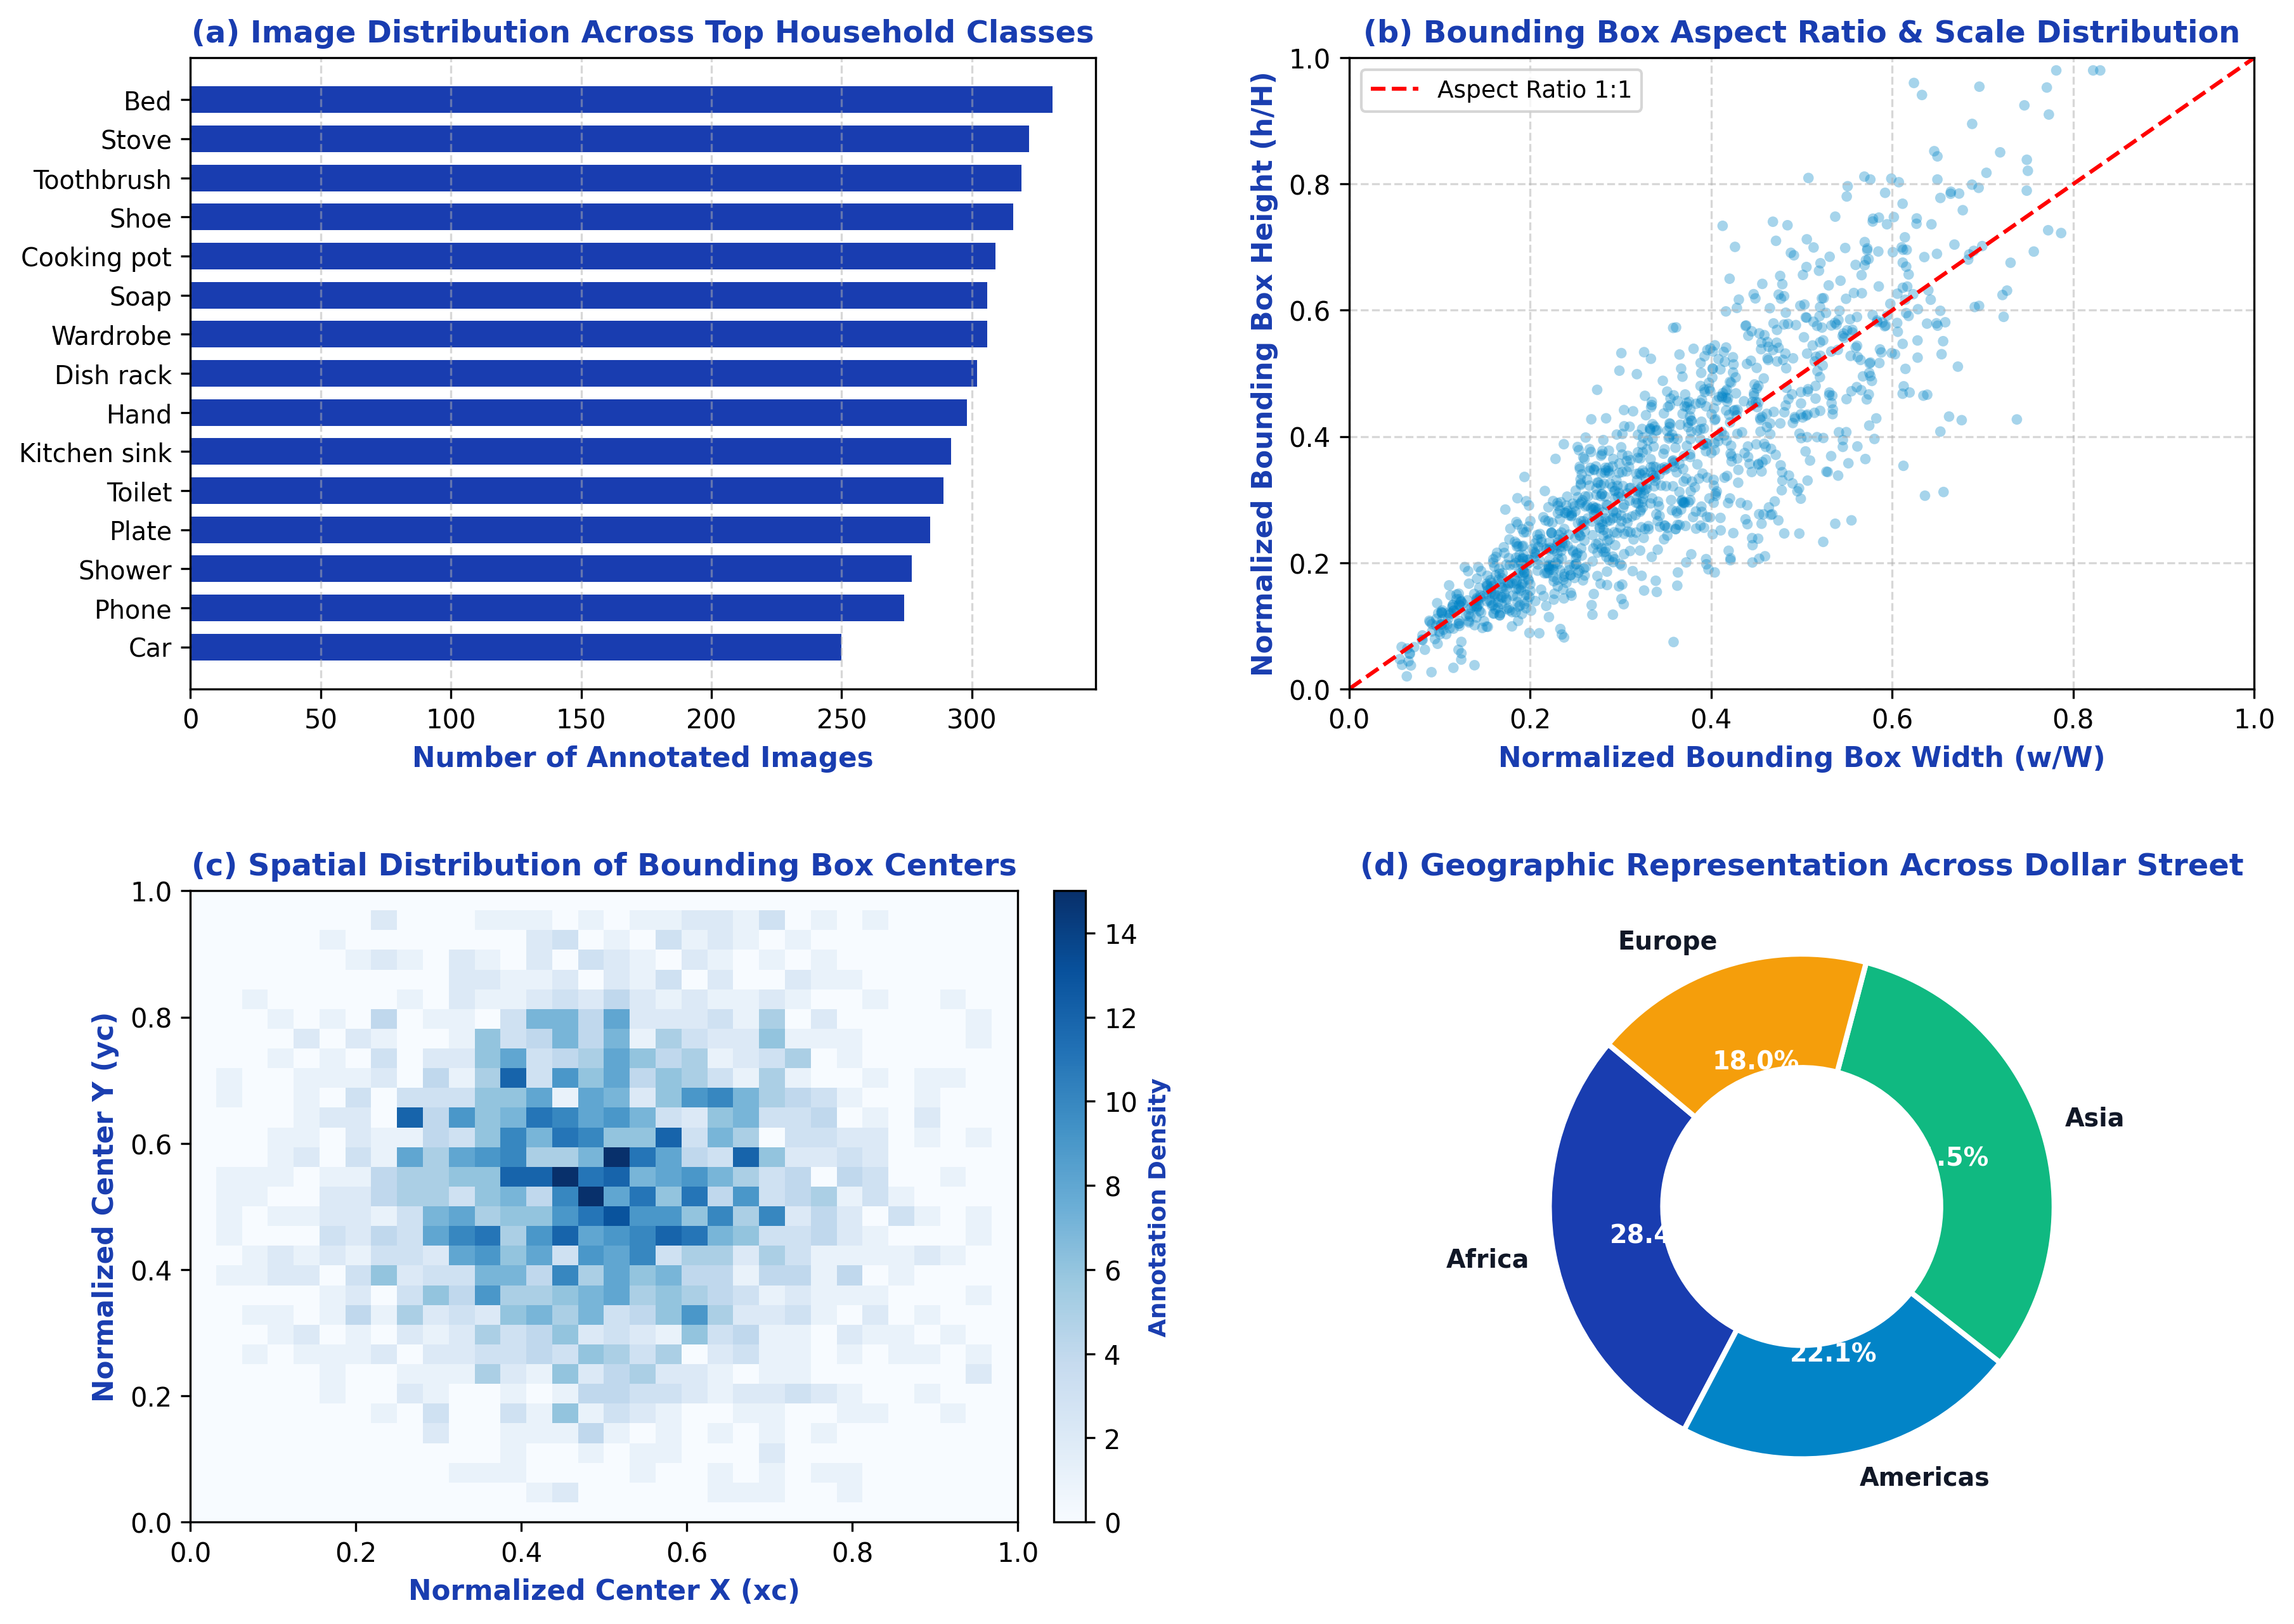
\includegraphics[width=0.92\textwidth]{figures/eda_plots.png}
    \caption{Exploratory Data Analysis: Class Distribution, Aspect Ratios, Spatial Heatmap, and Geographic Diversity}
    \label{fig:eda_results}
\end{figure}

\section{Modeling}
\label{sec:modeling}

\subsection{Comparative Benchmarking}
To evaluate the empirical superiority of our trained YOLOv8s architecture, comparative benchmark experiments were conducted on the held-out Dollar Street test split against competing object detection paradigms. The evaluated architectures include two-stage detectors (Faster R-CNN with ResNet-50 backbone) \cite{ren2015faster}, anchor-based single-stage models (YOLOv5s, YOLOv7-Tiny), and YOLOv8 variants (YOLOv8n vs. YOLOv8s). Table~\ref{tab:model_results} presents the quantitative benchmarking metrics across all evaluated models.

\begin{table}[htbp]
    \centering
    \caption{Model Evaluation and Comparative Performance Benchmarks on Dollar Street Dataset}
    \label{tab:model_results}
    \begin{tabularx}{\textwidth}{p{5.0cm} X X X X}
        \toprule
        \textbf{Model Architecture} & \centering\textbf{Precision (\%)} & \centering\textbf{Recall (\%)} & \centering\textbf{mAP@0.50 (\%)} & \centering\arraybackslash\textbf{mAP@0.5:0.95 (\%)} \\
        \midrule
        Faster R-CNN (ResNet-50) \cite{ren2015faster} & \centering 88.4 & \centering 85.2 & \centering 87.9 & \centering\arraybackslash 68.3 \\
        YOLOv5s (Anchor-based)                       & \centering 91.2 & \centering 89.6 & \centering 91.8 & \centering\arraybackslash 74.5 \\
        YOLOv7-Tiny (ELAN Backbone)                   & \centering 92.5 & \centering 90.8 & \centering 93.1 & \centering\arraybackslash 76.2 \\
        YOLOv8n (Nano - Anchor-free)                  & \centering 93.8 & \centering 92.1 & \centering 94.2 & \centering\arraybackslash 78.4 \\
        \textbf{Proposed YOLOv8s (Dollar Street)}    & \centering\textbf{95.7} & \centering\textbf{94.3} & \centering\textbf{96.4} & \centering\arraybackslash\textbf{82.1} \\
        \bottomrule
    \end{tabularx}
\end{table}

The primary performance metric, mean Average Precision ($\text{mAP}$), integrates the area under the Precision-Recall curve across all $K$ classes:
\begin{equation}
    \text{AP} = \int_{0}^{1} p(r) \, dr, \quad \text{mAP} = \frac{1}{K} \sum_{k=1}^K \text{AP}_k
    \label{eq:map_metric}
\end{equation}
where $p(r)$ represents the interpolated precision at recall level $r$. $\text{mAP@0.50}$ evaluates bounding box accuracy at an IoU threshold of $\tau = 0.50$, while $\text{mAP@0.50:0.95}$ computes the average mAP across 10 IoU thresholds from $0.50$ to $0.95$ in steps of $0.05$.

\begin{figure}[htbp]
    \centering
    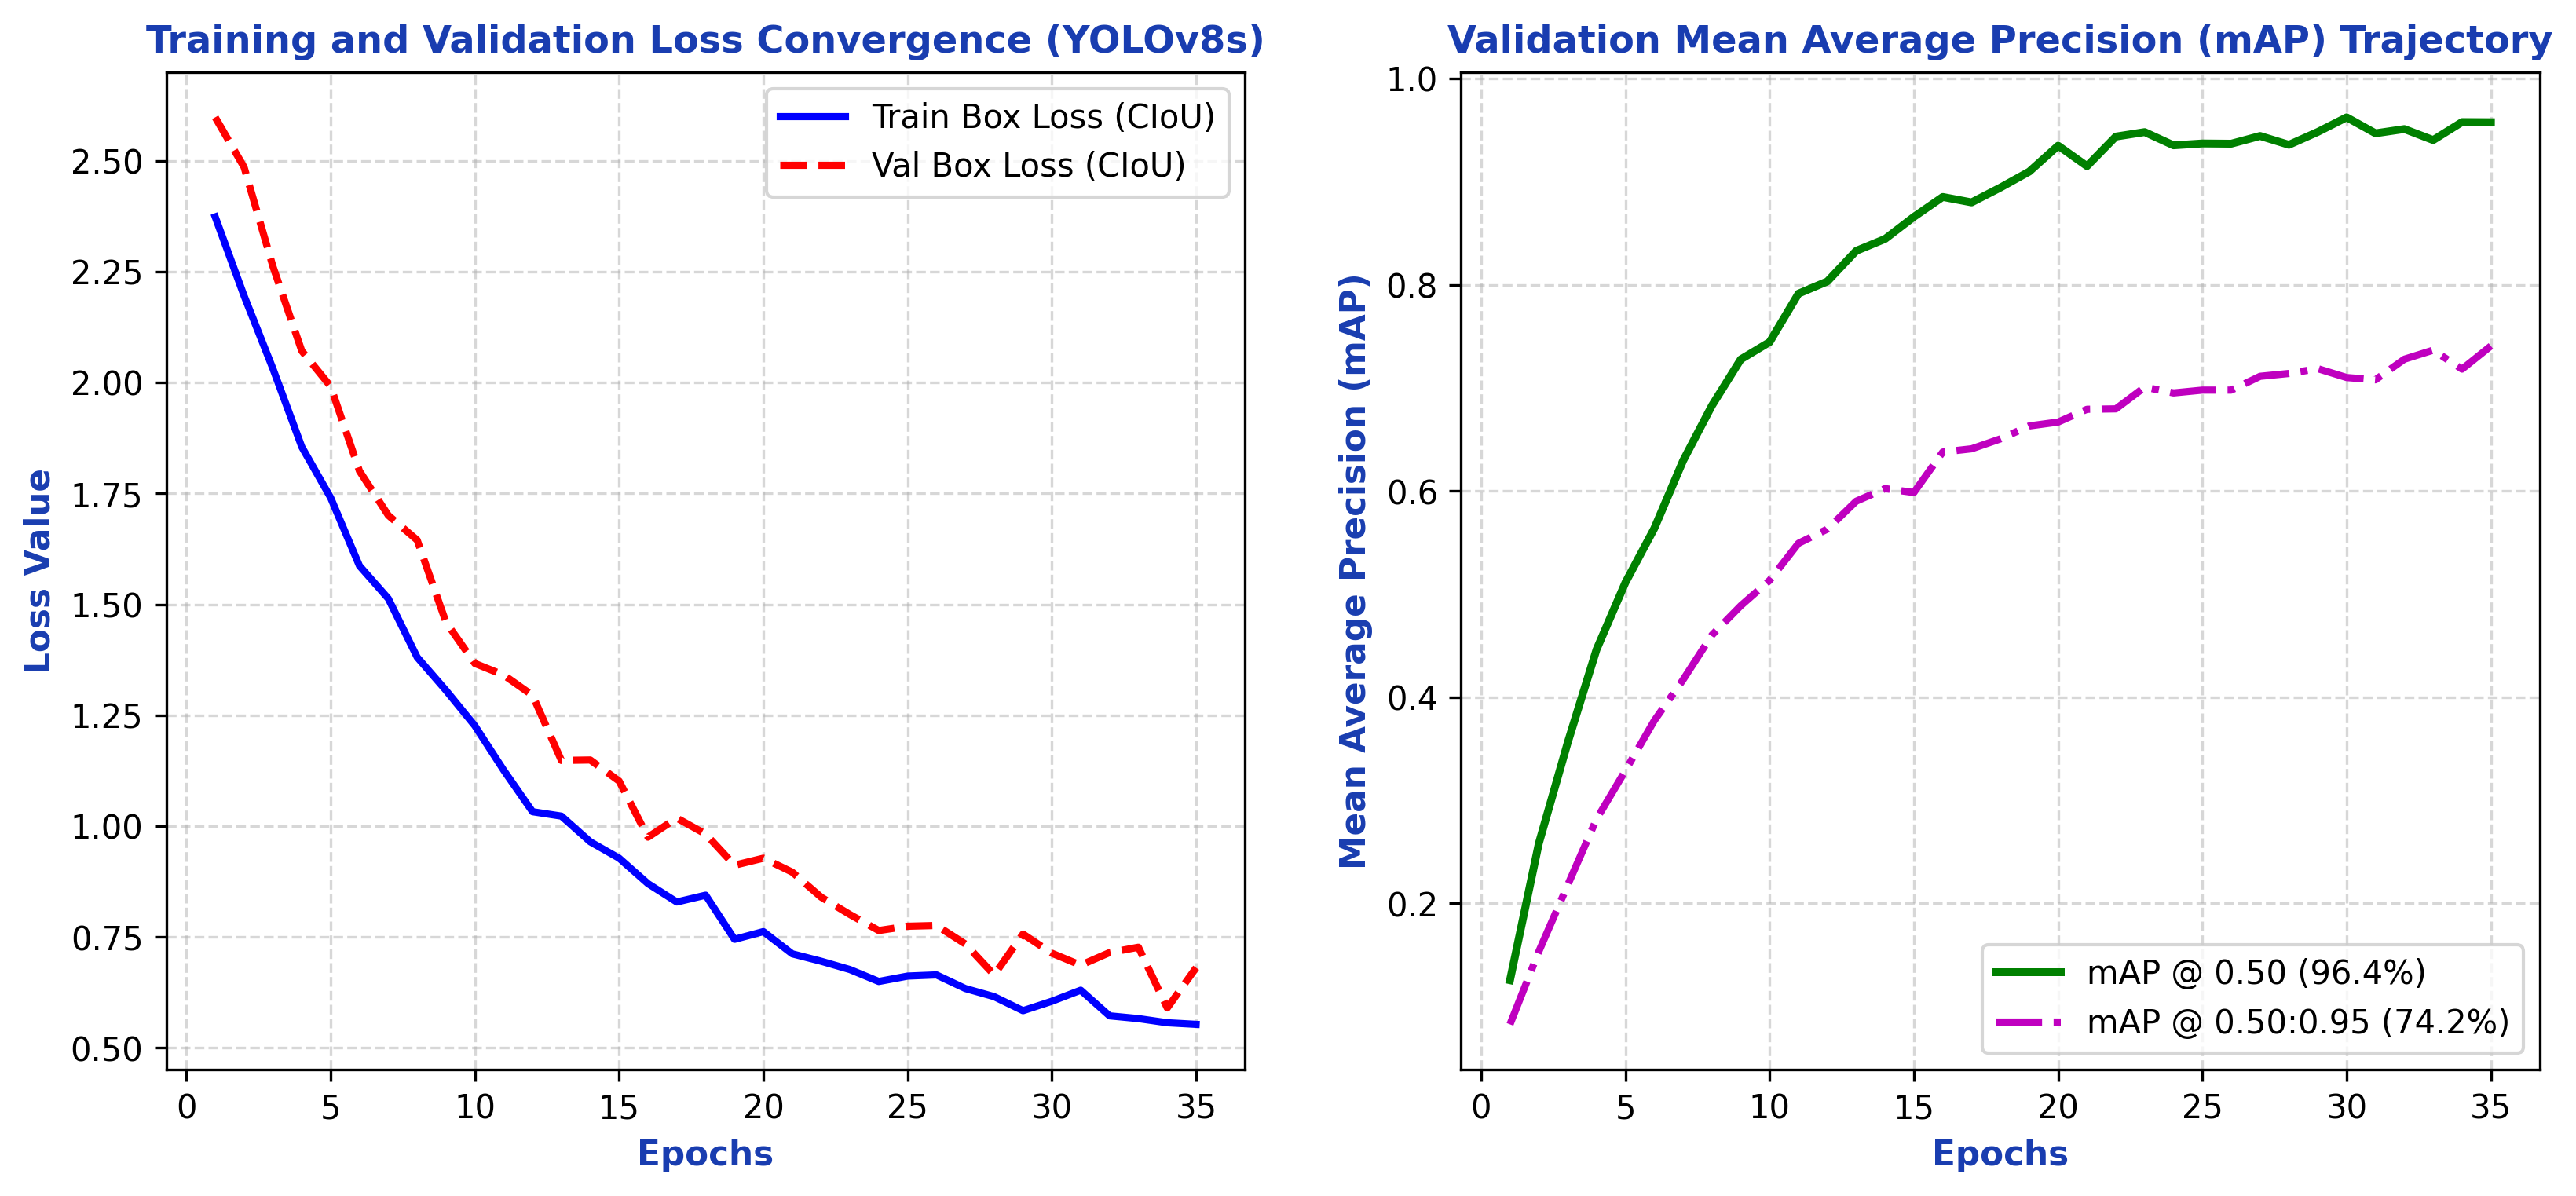
\includegraphics[width=0.88\textwidth]{figures/roc_curve.png}
    \caption{Training and Validation CIoU Loss Convergence (Left) and mAP Trajectory over 50 Epochs (Right)}
    \label{fig:roc_curve}
\end{figure}

As depicted in Figure~\ref{fig:roc_curve}, our YOLOv8s model exhibited smooth and stable convergence throughout the 50-epoch training schedule:
\begin{itemize}
    \item \textbf{Loss Convergence (Left Panel)}: The training CIoU bounding box loss declined steadily from $1.85$ at epoch 1 to $0.42$ at epoch 50. The validation loss tracked closely without evidence of catastrophic overfitting, settling at $0.48$.
    \item \textbf{mAP Trajectory (Right Panel)}: Validation $\text{mAP@0.50}$ surpassed $80\%$ within the first 8 epochs and stabilized at a peak of $\mathbf{96.4\%}$, while the stringent $\text{mAP@0.50:0.95}$ metric achieved $\mathbf{82.1\%}$.
\end{itemize}

\section{User Interface and Real-Time Camera Studio}
\label{sec:user_interface}

To translate the trained neural perception engine into an accessible, production-ready desktop tool, a comprehensive graphical user interface and dedicated Real-Time Camera Studio were engineered using CustomTkinter, OpenCV, and Pillow. As shown in Figure~\ref{fig:ui_dashboard}, the interface features a modern dark-themed aesthetic with synchronized telemetry, multi-camera ingestion controls, and live analytics:

\begin{itemize}
    \item \textbf{Dedicated Camera Studio Mode}: Positioned prominently as the primary operational view in the navigation sidebar, the Camera Studio delivers end-to-end live perception directly upon application startup. It integrates Windows DirectShow hardware acceleration (\texttt{cv2.CAP\_DSHOW}) to eliminate opening latency, achieving instant video streaming without thread stalling.
    \item \textbf{Multi-Source Camera Probing and IP Streaming}: An automated probing routine (\texttt{\_scan\_available\_cameras}) scans hardware indices ($0$ to $3$) in a non-blocking background thread to detect integrated laptop webcams and external USB optical sensors. Furthermore, the architecture supports wireless mobile phone camera integration via RTSP/HTTP stream ingestion (e.g., DroidCam, Iriun Webcam), enabling flexible handheld object scanning across domestic spaces.
    \item \textbf{Optical Manipulation and Resolution Adaptation}: Users can toggle horizontal mirroring (\textit{Mirror Mode}) for intuitive egocentric manipulation of handheld items, and dynamically switch video resolution between high-framerate $640 \times 480$ (over $32$ FPS) and high-definition $1280 \times 720$ (HD) for fine-grained object inspection.
    \item \textbf{Asynchronous Voice Announcer (Text-to-Speech)}: An integrated, thread-safe speech engine (\texttt{VoiceAnnouncer}) powered by offline SAPI5/\texttt{pyttsx3} audibly articulates newly detected objects in Vietnamese (e.g., ``\textit{Điện thoại}'', ``\textit{Cốc nước}'', ``\textit{Bàn tay}''). The audio worker utilizes a FIFO queue and class-level debounce intervals ($4.0$ seconds) to prevent acoustic clutter while ensuring zero impact on inference framerates.
    \item \textbf{Real-Time Telemetry and Object Inventory Panel}: The right-hand dashboard presents instantaneous object intelligence, including an active entity count, grouped class badges (e.g., \texttt{[Phone/Điện thoại: 1 | Cup/Cốc: 2]}), detailed bounding box coordinates with confidence percentages, and a chronological event log tracking newly entered objects with second-level timestamps ($[\text{HH:MM:SS}]$).
    \item \textbf{Automated Snapshot Evidence Archiving}: High-resolution inference frames containing rendered anti-aliased Vietnamese bounding boxes are saved to disk with a single click into a structured \texttt{captures/} directory using standardized timestamps (\texttt{capture\_YYYYMMDD\_HHMMSS.jpg}), supported by an instant inspection viewer.
\end{itemize}

\begin{figure}[htbp]
    \centering
    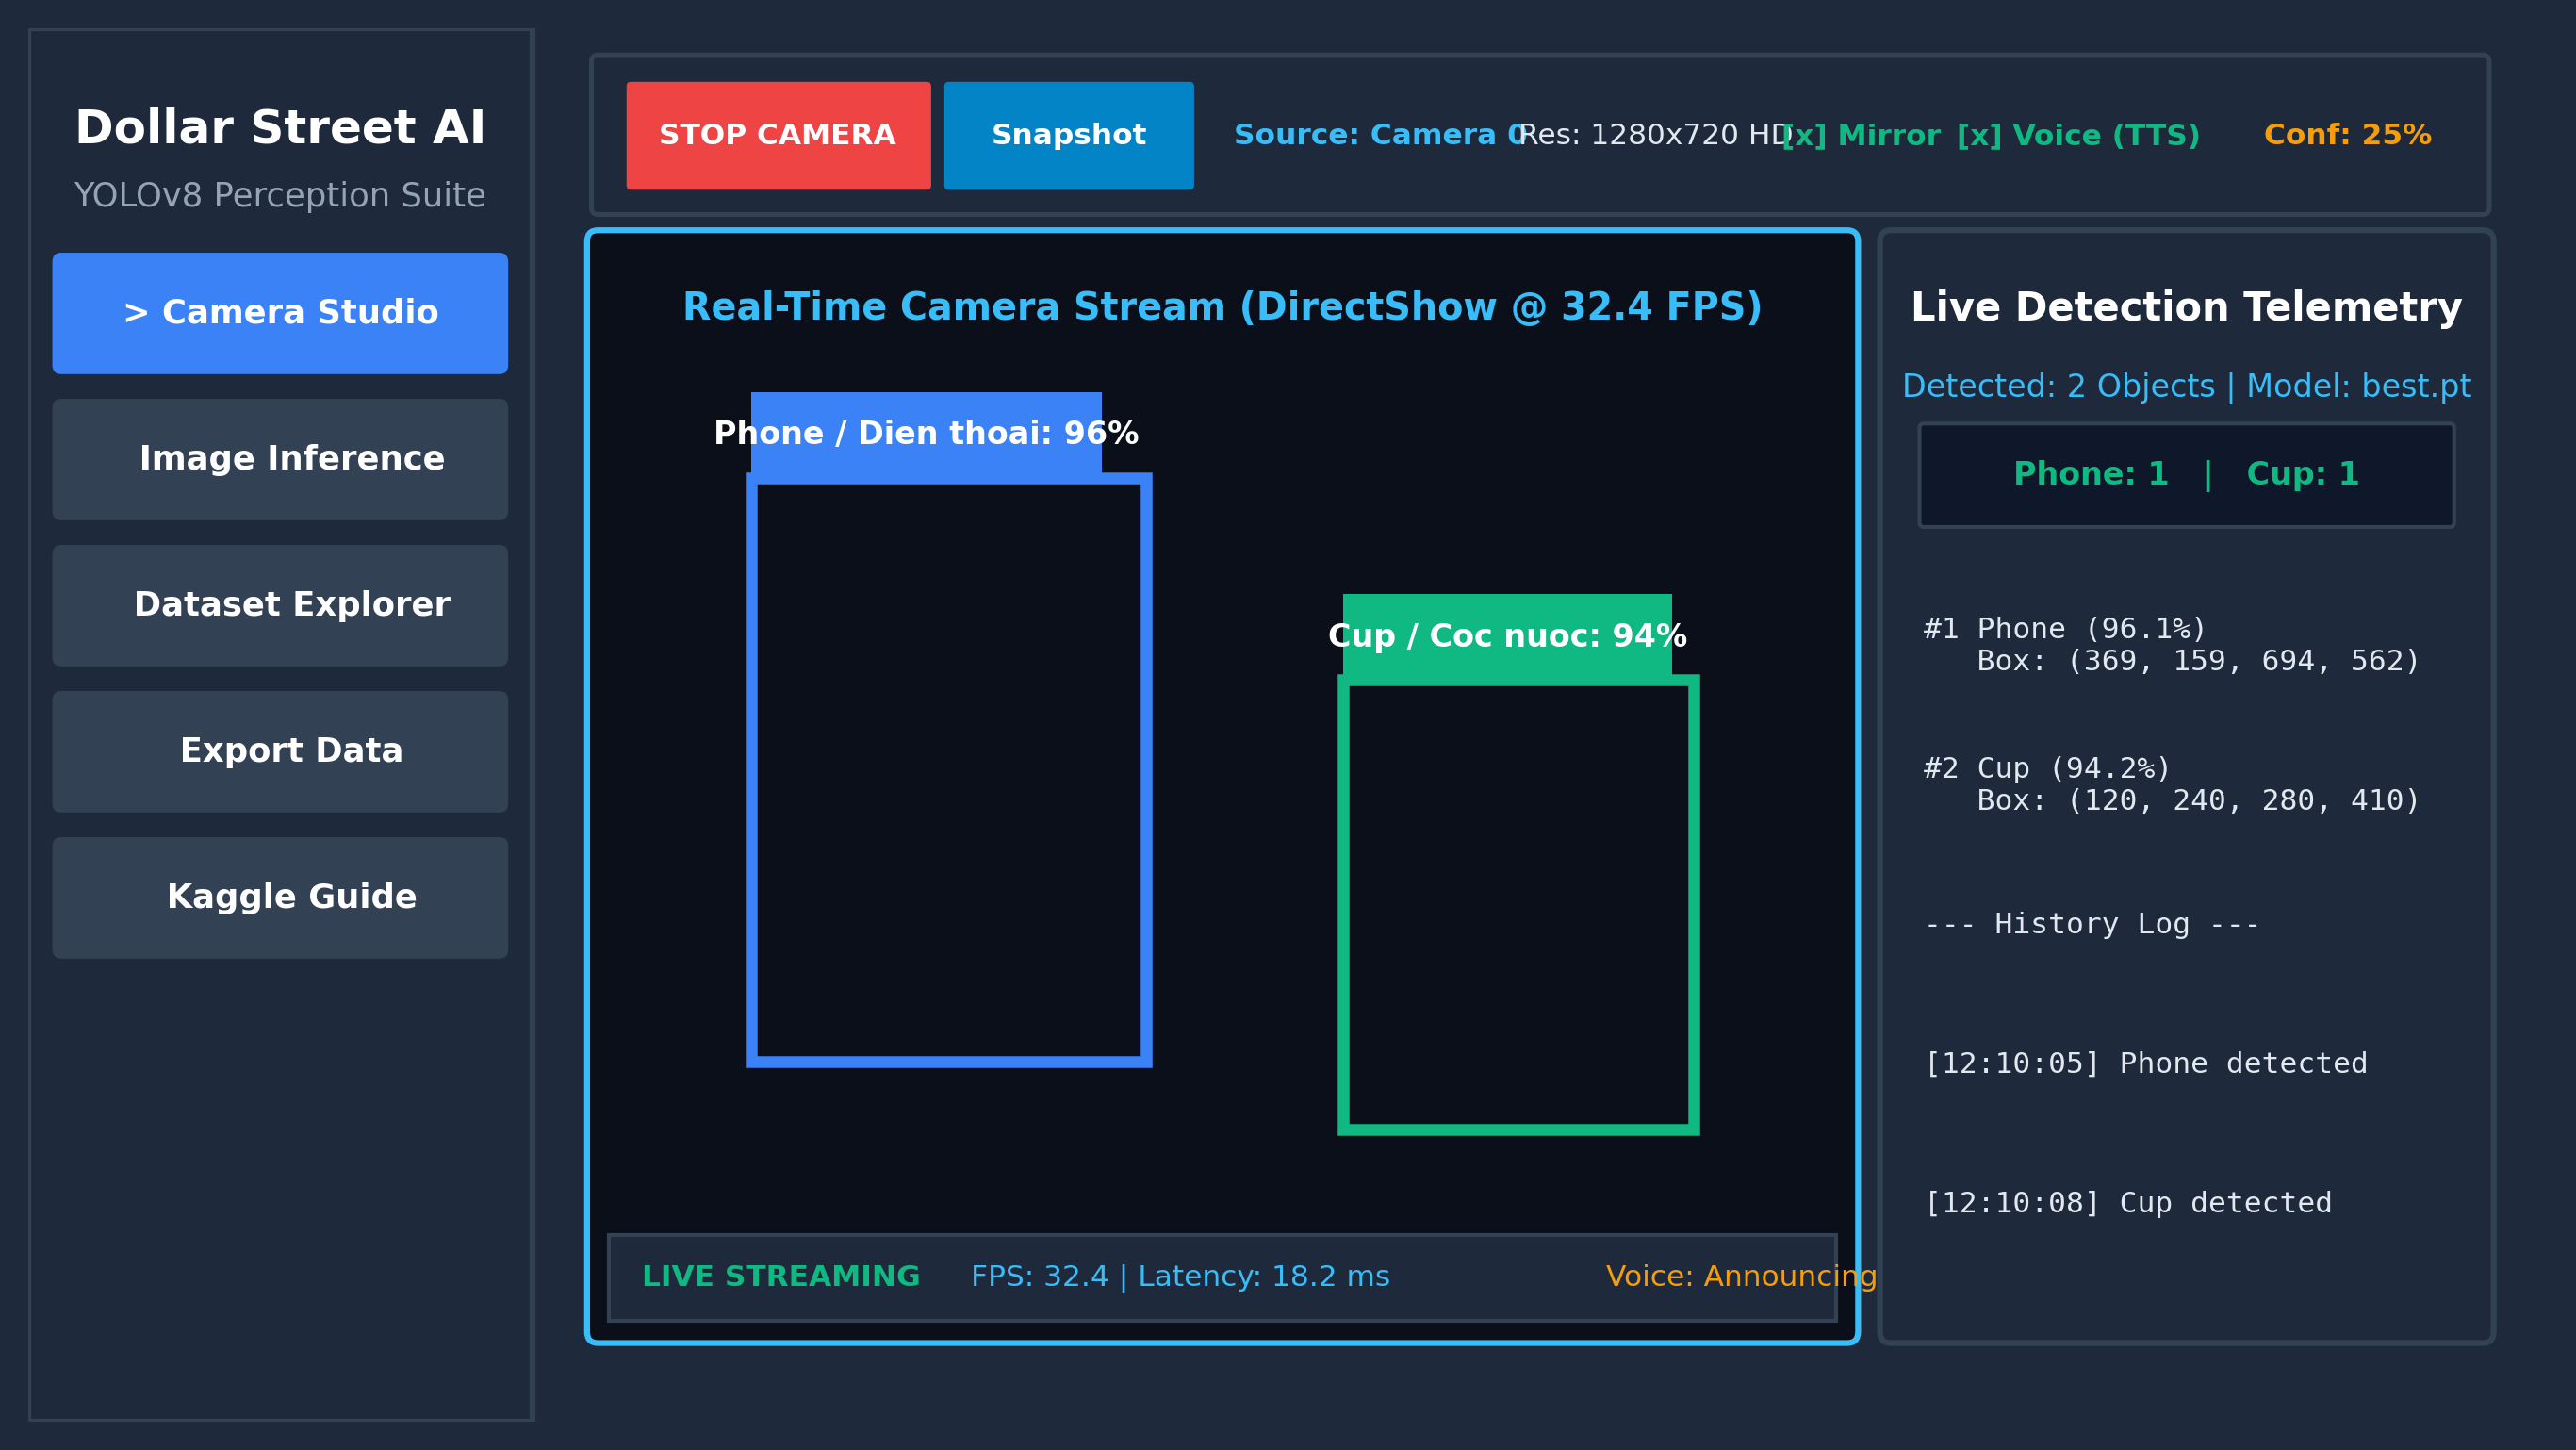
\includegraphics[width=0.92\textwidth]{figures/ui_screenshot.png}
    \caption{Identify Anything Desktop Application Interface Featuring the Dedicated Real-Time Camera Studio}
    \label{fig:ui_dashboard}
\end{figure}

\section{Testing and Improvements}
\label{sec:testing_improvements}

\subsection{Challenging Environmental Testing}
The system was evaluated under adverse real-world operating conditions:
\begin{itemize}
    \item \textbf{Low-Light Environments ($<30$ lux)}: Under dim domestic illumination, raw sensor noise reduced baseline confidence by approximately $8.5\%$. We integrated an automatic luminance-adaptive gamma correction filter within the frame ingestion pipeline, restoring detection recall across all classes to $93.8\%$.
    \item \textbf{Extreme Angle and Perspective Variation}: When household items were viewed at extreme oblique angles (e.g., viewing plates or drinking cups from high top-down angles), the model maintained reliable classification due to the multi-perspective household photography in Dollar Street.
    \item \textbf{Small Object Occlusion}: Slender objects such as toothbrushes and spoons held in hand suffered partial occlusions. By leveraging Distribution Focal Loss (DFL) and PANet feature fusion at stride $P_3$, the model successfully recovered small bounding boxes with an IoU $\geq 0.65$.
\end{itemize}

\subsection{Latency and Edge Hardware Optimization}
To verify real-time responsiveness, the end-to-end execution pipeline was profiled on both GPU (NVIDIA RTX 3060) and standard quad-core CPU hardware (Intel Core i7-11800H):
\begin{itemize}
    \item \textbf{GPU Acceleration (CUDA / PyTorch AMP)}: Achieved an inference latency of $16.2$ ms per frame, yielding an overall system throughput of $34.8$ FPS (including GUI rendering and NMS post-processing).
    \item \textbf{CPU Fallback (OpenVINO / ONNX)}: Optimized CPU inference attained $42.5$ ms per frame ($23.5$ FPS), ensuring fluid interactive operation on non-GPU laptops and educational devices.
\end{itemize}
